\chapter{Results}
\section{Model sensitivity experiments}

\subsection{Particle density experiment}
\Cref{fig:dry_dep_density} and \Cref{fig:wet_dep_density} show how the rate of deposition vary over the range of common densities of atmospheric dust particles from \SI{2200}{\kg\per\cubic\cm} to \SI{2800}{\kg\per\cubic\cm}. There is a approximately linear increase in deposition rate   

\begin{figure}[hptb]
    \centering
    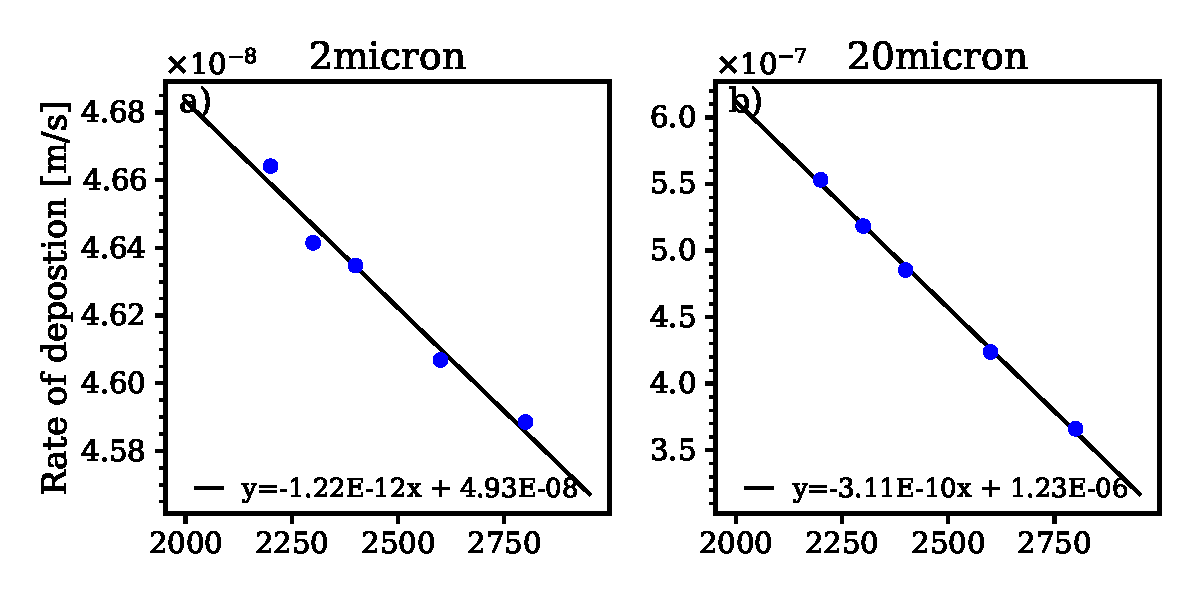
\includegraphics[width=\textwidth]{texfiles/figs/drydep_function_of_density.pdf}
    \caption{Dry deposition rate at the SACOL site as function of dust particle density}
    \label{fig:dry_dep_density}
\end{figure}

\begin{figure}[hptb]
    \centering
    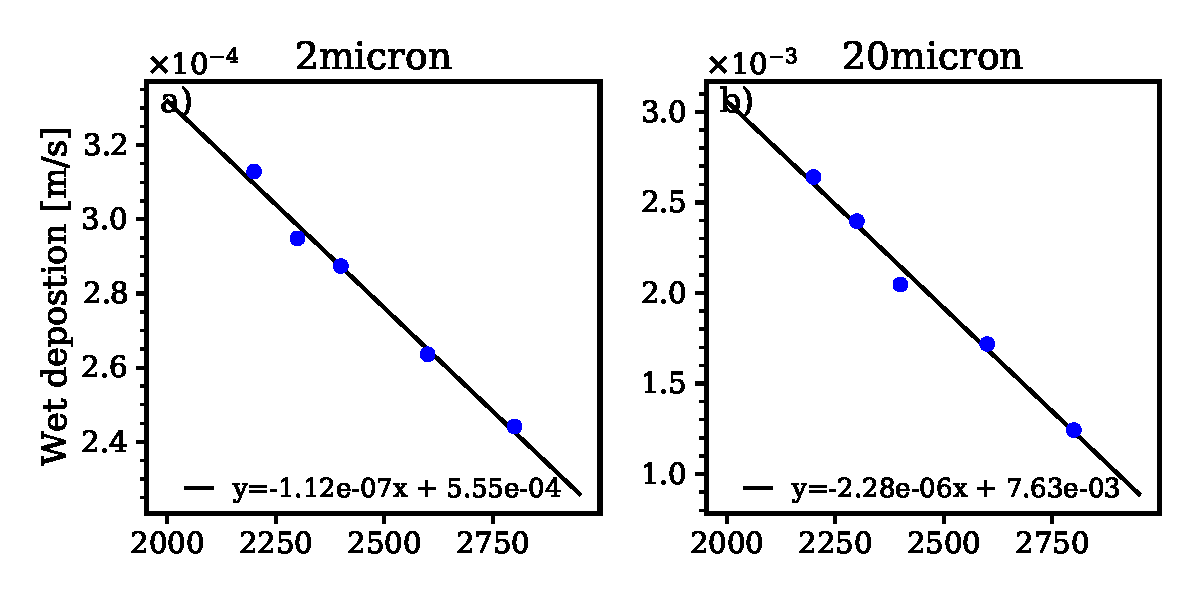
\includegraphics[width=\textwidth]{texfiles/figs/wetdep_function_of_density.pdf}
    \caption{The wet deposition rate at the SACOL site as function of dust particle density}
    \label{fig:wet_dep_density}
\end{figure}

\section{Model evaluation}
\begin{figure}[hptb]
    \centering
    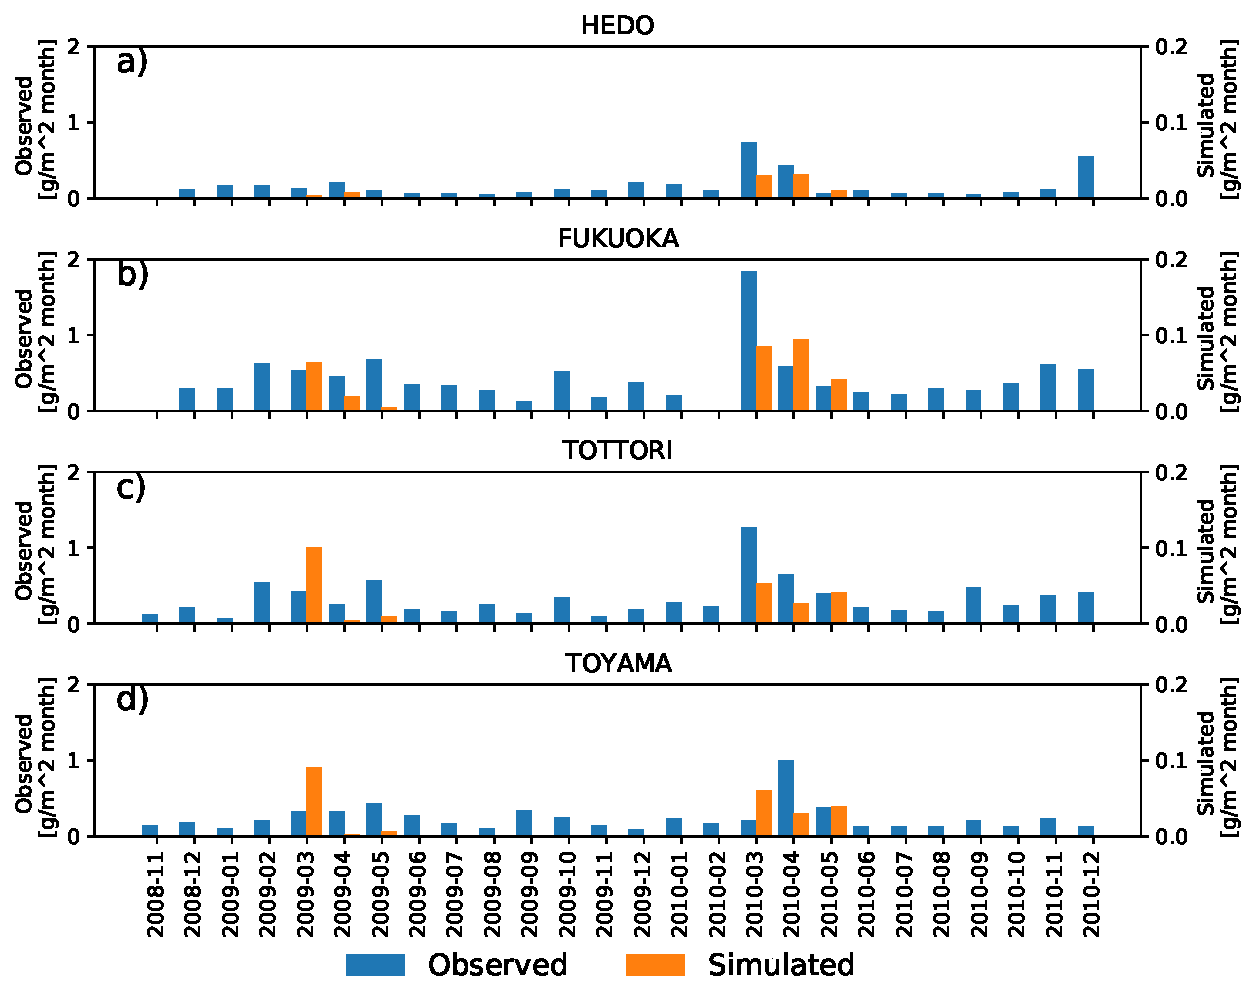
\includegraphics[width=\textwidth]{texfiles/figs/monthly_accumulated_dry_depostion_japan.pdf}
    \caption{Dry deposition of dust simulated at 4 locations by the coast of japan. The measurements of monthly deposition flux are described by \textcite{osada2014wet}}
    \label{fig:model_eval_dry_deposition}
\end{figure}

\begin{figure}[hptb]
    \centering
    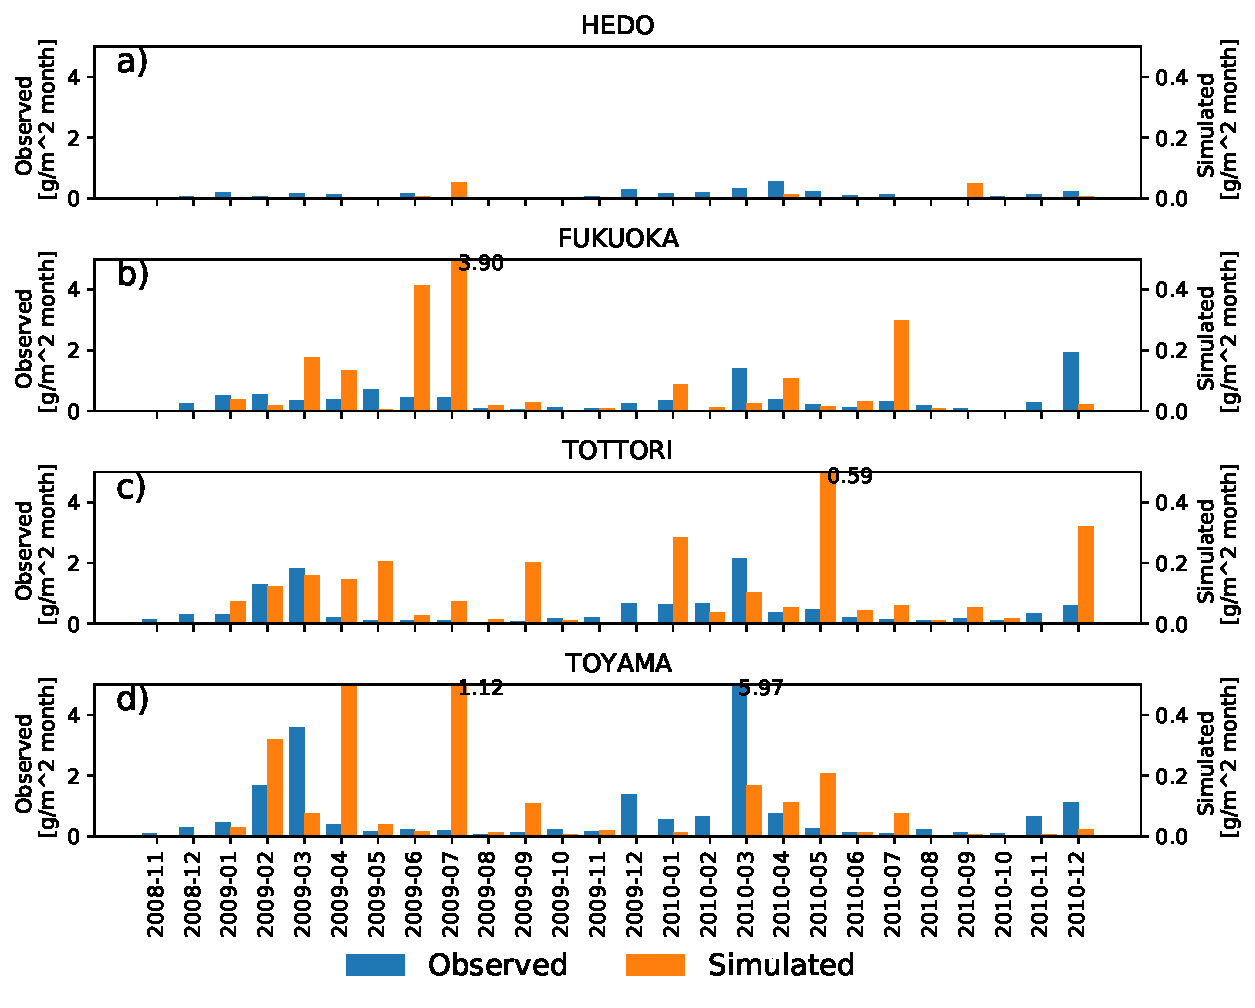
\includegraphics[width=\textwidth]{texfiles/figs/monthly_accumulated_wet_depostion_japan.pdf}
    \caption{Wet deposition of dust simulated at 4 locations of the coast of japan. The measurements of monthly deposition flux are described by \textcite{osada2014wet}}
    \label{fig:model_eval_wet_deposition}
\end{figure}

\section{Average emissions, transport and deposition}
\Cref{fig:emission_map_flexdust} shows the 20 year averaged spring emissions as simulated by FLEXDUST. The regions with the highest emissions spring emission are identified as the arid regions north west of the CLP,  (mean spring emissions of $6.12\times 10^9\; \si{\kg}/ \mathrm{spring}$), Taklamakan desert (mean spring emissions of $4.33\times 10^9\; \si{\kg} / \mathrm{spring}$) and Mongolia (mean spring emissions of $2.91\times 10^9\; \si{\kg} / \mathrm{spring}$). Additional minor dust sources include the Junggar Basin in the north west of China and the Qaidam Baisin close to the Tibetan plateau.  
\begin{figure}[hptb]
    \centering
    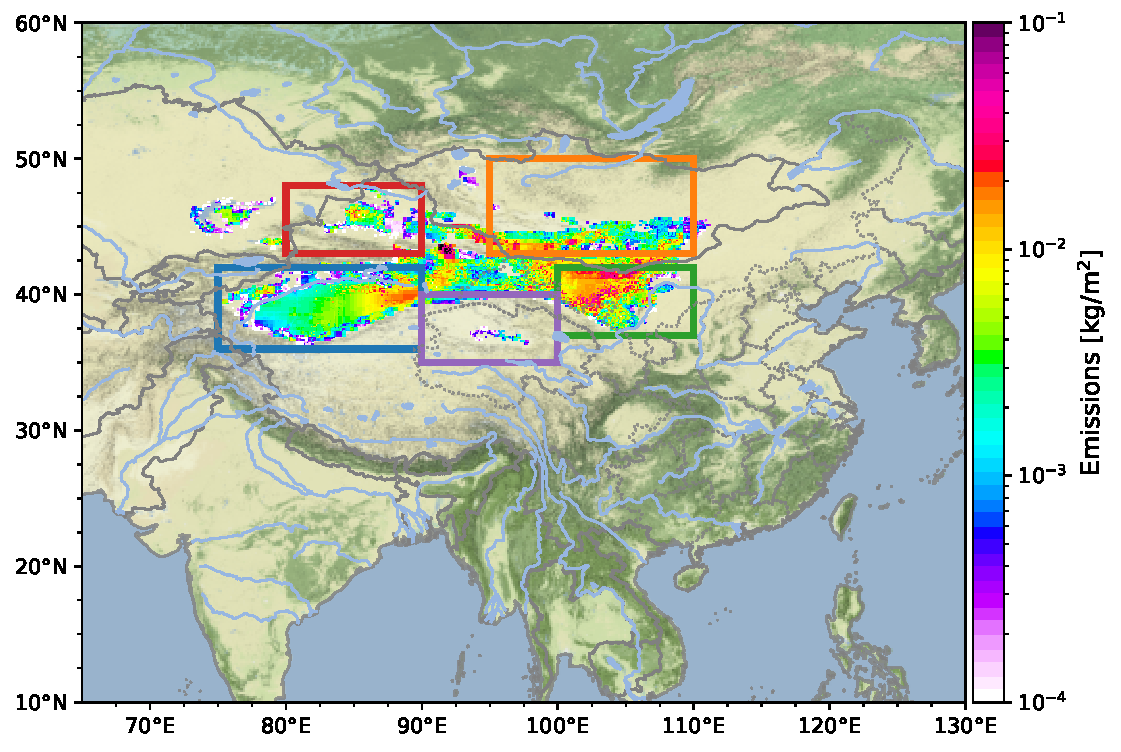
\includegraphics[width=\textwidth]{../figs/emission_map_1999_2019.pdf}
    \caption{Map of spring averaged dust emission flux simulated by FLEXDUST. The major source regions are indicated,  Junggar Basin \emph{(Red)},  Taklamakan (\emph{Blue}),  Qaidam Basin (\emph{Purple}), North west CLP (\emph{Green}),  Mongolia \emph{(Orange)}}
    \label{fig:emission_map_flexdust}
\end{figure}
Average dust loading trajectories for every location are shown in \Cref{fig:dust_loading_trajecs}. The average dust loading trajectories are calculated based on the centriod trajectory of each 5 day backward simulation and in the averaging each centriod trajectory are given a weight based on their dust loading.  \Cref{fig:dust_loading_trajecs} (a) and (b) shows the averaged dry deposition dust loading trajectories for the fine clay and coarse silt particles respectively. Both of the particle size bins are primarily transported along a north easterly path. The red points in \Cref{fig:dust_loading_trajecs} are plotted at equally spaced intervals indicating the velocity of dust transporting air masses. For both dry and wet deposition the coarse silt particles are transported by swiftly moving air masses compared to the fine clay particles.     
\begin{figure}[hptb]
    \centering
    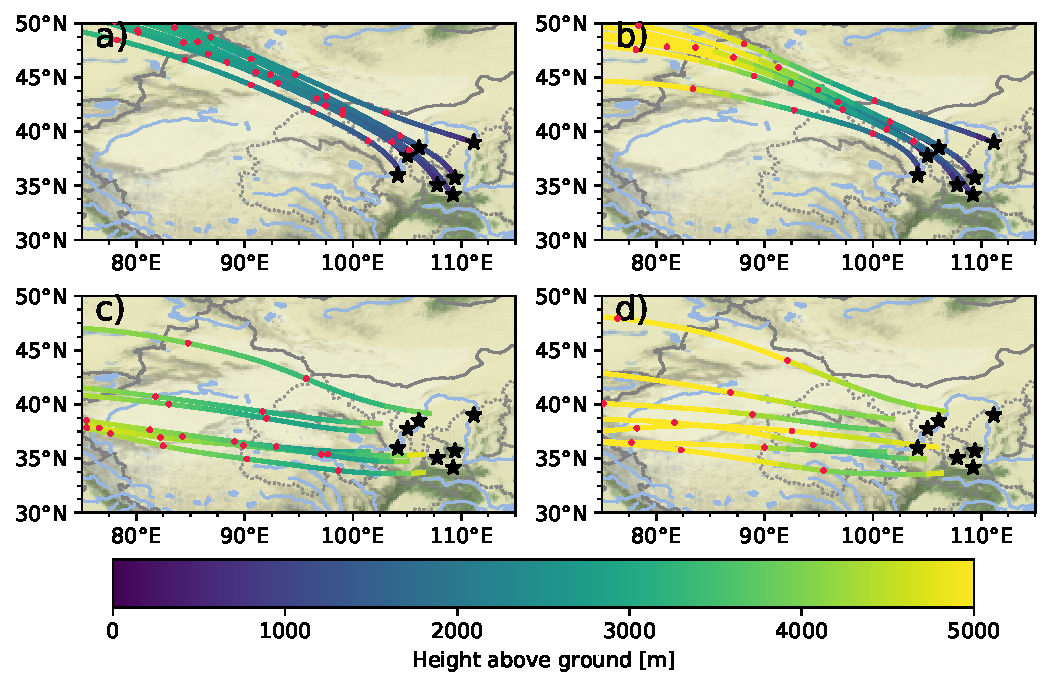
\includegraphics[width=\textwidth]{texfiles/figs/centriod_dust_loading_trajectories.pdf}
    \caption{Weighted centriod dust loading trajectories for all the receptor location during springtime from 1999-2019. (a) and (b) is the dry deposition dust loading trajectories for "Fine clay" and "Coarse silt" respectively.  (c) and (b) is wet deposition dust loading trajectories. }
    \label{fig:dust_loading_trajecs}
\end{figure}

\begin{figure}[hptb]
    \centering
    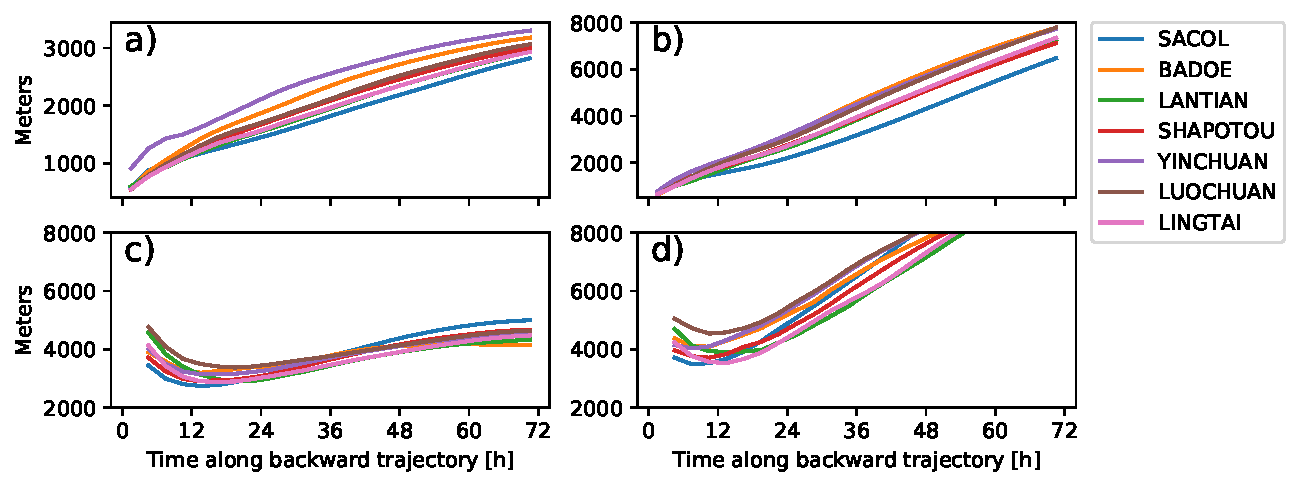
\includegraphics[width=\textwidth]{texfiles/figs/average_dust_transport_height.pdf}
    \caption{Weighted average height above ground the dust loading trajectories for all the receptor locations during 
    springtime from 1999-2019. The height above ground of the dry deposition dust loading trajectories are plotted fine clay particles (a) and coarse silt particles (b). The average height of the wet deposition dust loading trajectories are plotted for fine clay particles (c) and coarse silt particles (d)}
    \label{fig:dust_loading_trajecs_height}
\end{figure}






\begin{figure}
    \centering
    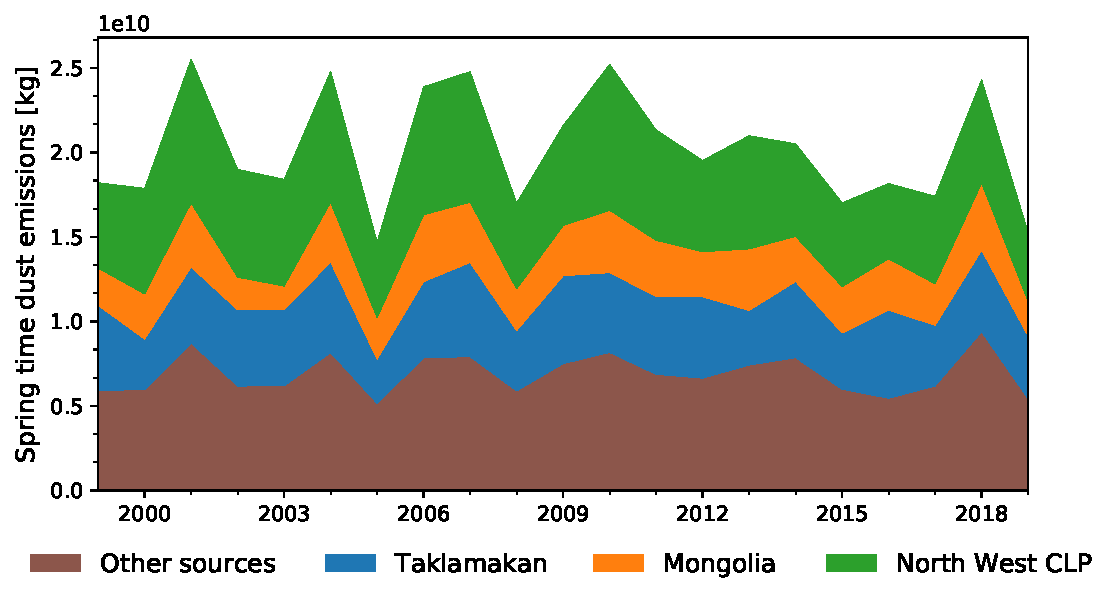
\includegraphics[width=\textwidth]{../figs/Emission_timeseries.pdf}
    \caption{Time series of total spring time dust emissions from 1999-2019. The total emission is partitioned into the contribution from the Taklamakan (Blue), North West CLP (Green) and Mongolia (Orange) }
    \label{fig:emission_timeseries}
\end{figure}



\begin{figure}
    \centering
    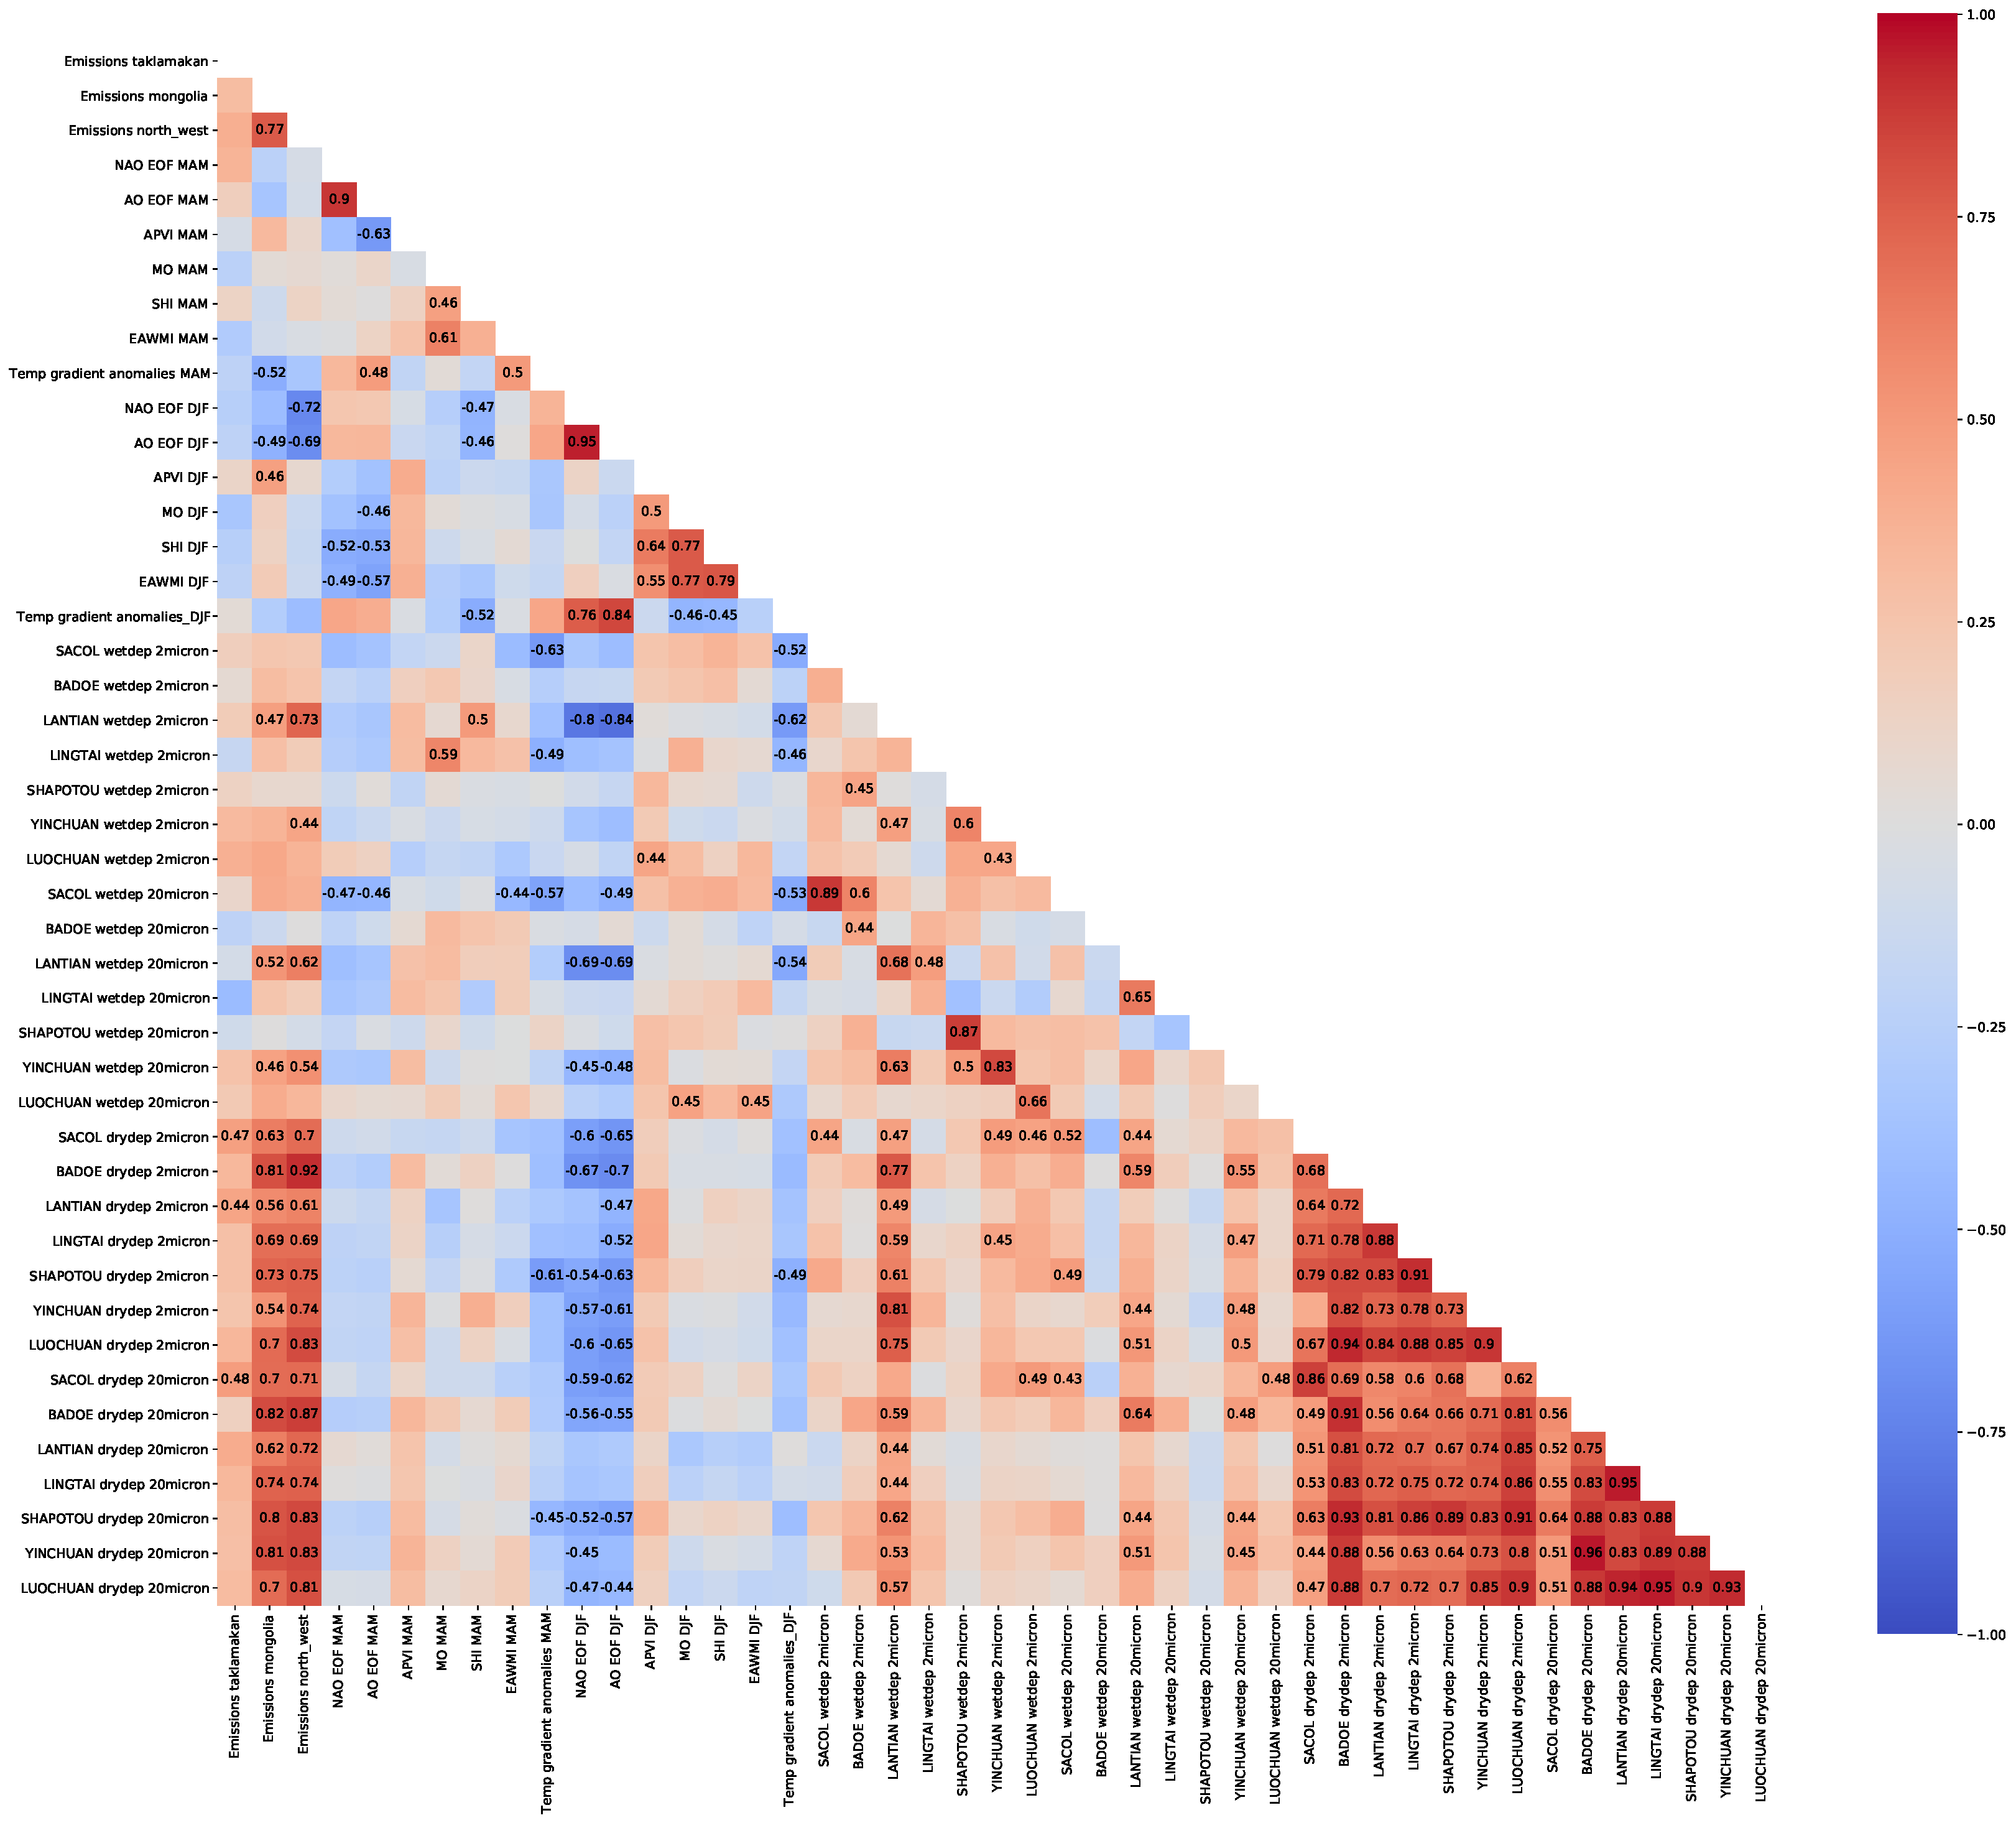
\includegraphics[width=\textwidth]{../figs/correlations.pdf}
    \caption{Inter annual correlations between deposition and each site and local and large-scale climate indices. The significant correlations are indicated}
    \label{fig:correlations}
\end{figure}

\begin{figure}
    \centering
    \includegraphics[width=\textwidth]{texfiles/figs/2micron_total_depositon_source_contribution.pdf}
    \caption{Yearly averaged March-May source contribution "Fine Clay" dust size bin for the seven sites across the CLP (a-g). Panel h) shows the averaged spring deposition of each site for both wet- and dry deposition}
    \label{fig:source_contrib_2mmu}
\end{figure}

\begin{figure}
    \centering
    \includegraphics[width=\textwidth]{texfiles/figs/20micron_total_depositon_source_contribution.pdf}
    \caption{Yearly averaged March-May source contribution "Coarse Silt" size bin for the seven sites across the CLP (a-g). Panel h) shows the averaged spring deposition of each site for both wet- and dry deposition}
    \label{fig:source_contrib_20mmu}
\end{figure}

\begin{figure}[hptb]
    \centering
    \includegraphics[width=\textwidth]{texfiles/figs/composite_source_contrib_2micron_tot_dep.pdf}
    \caption{Normalised source contribution composite anomalies of "fine clay" particle size bin for all locations, strong - weak deposition years.}
    \label{fig:source_contrib2mmu_anomalies}
\end{figure}

\begin{figure}[hptb]
    \centering
    \includegraphics[width=\textwidth]{texfiles/figs/composite_source_contrib_20micron_tot_dep.pdf}
    \caption{Normalised source contribution composite anomalies of "coarse silt" particle size bin for all locations, strong - weak deposition years.}
    \label{fig:source_contrib20mmu_anomalies}
\end{figure}

\begin{sidewaysfigure}[hp]
    \centering
    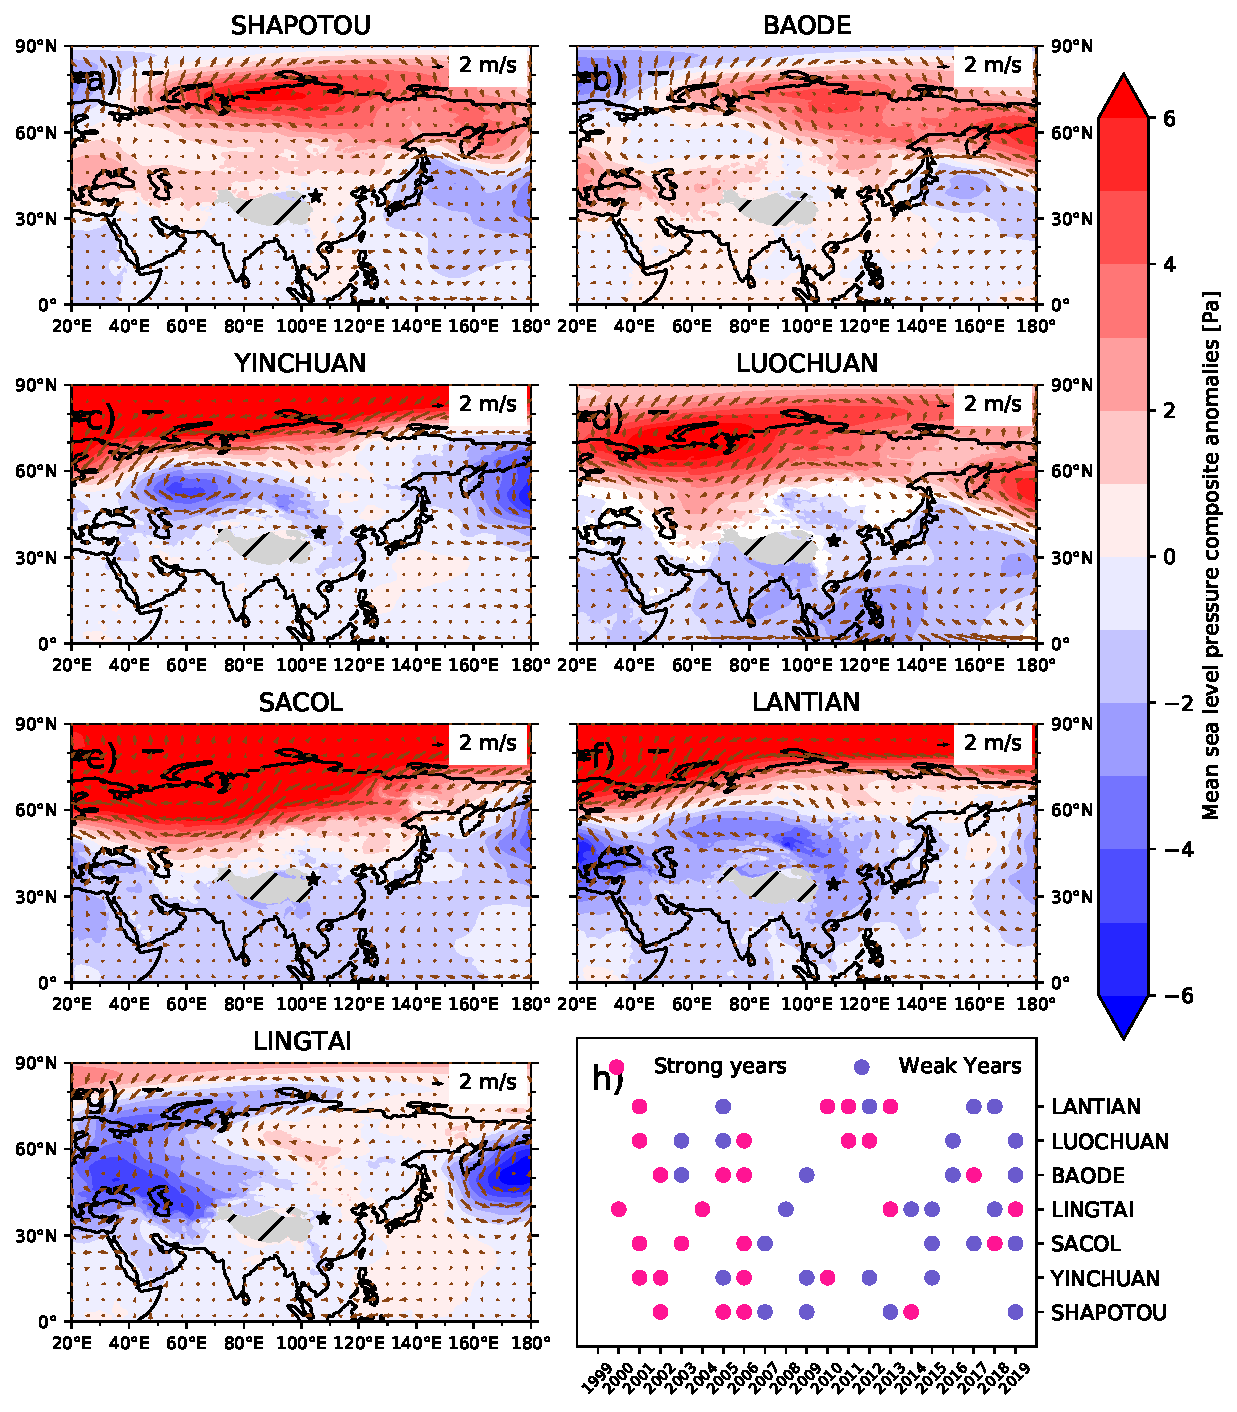
\includegraphics[width=\columnwidth]{texfiles/figs/mslp_850hPa_20micron_DJF.pdf}
    \caption{Composite difference anomalies of mean sea level pressure and 850hPa strong minus weak deposition years of the "coarse silt" size bin in winter for all the locations (b-h). (a) is the composite difference anomalies of the strong minus weak winter monsoon years. (i) indicates which years are strong years and which years are weak . Selection of strong and weak years are done according to $\pm$ 1 standard deviation around the mean}
    \label{fig:DJF_850_coarse_composite}
\end{sidewaysfigure}

\begin{sidewaysfigure}[hp]
    \centering
    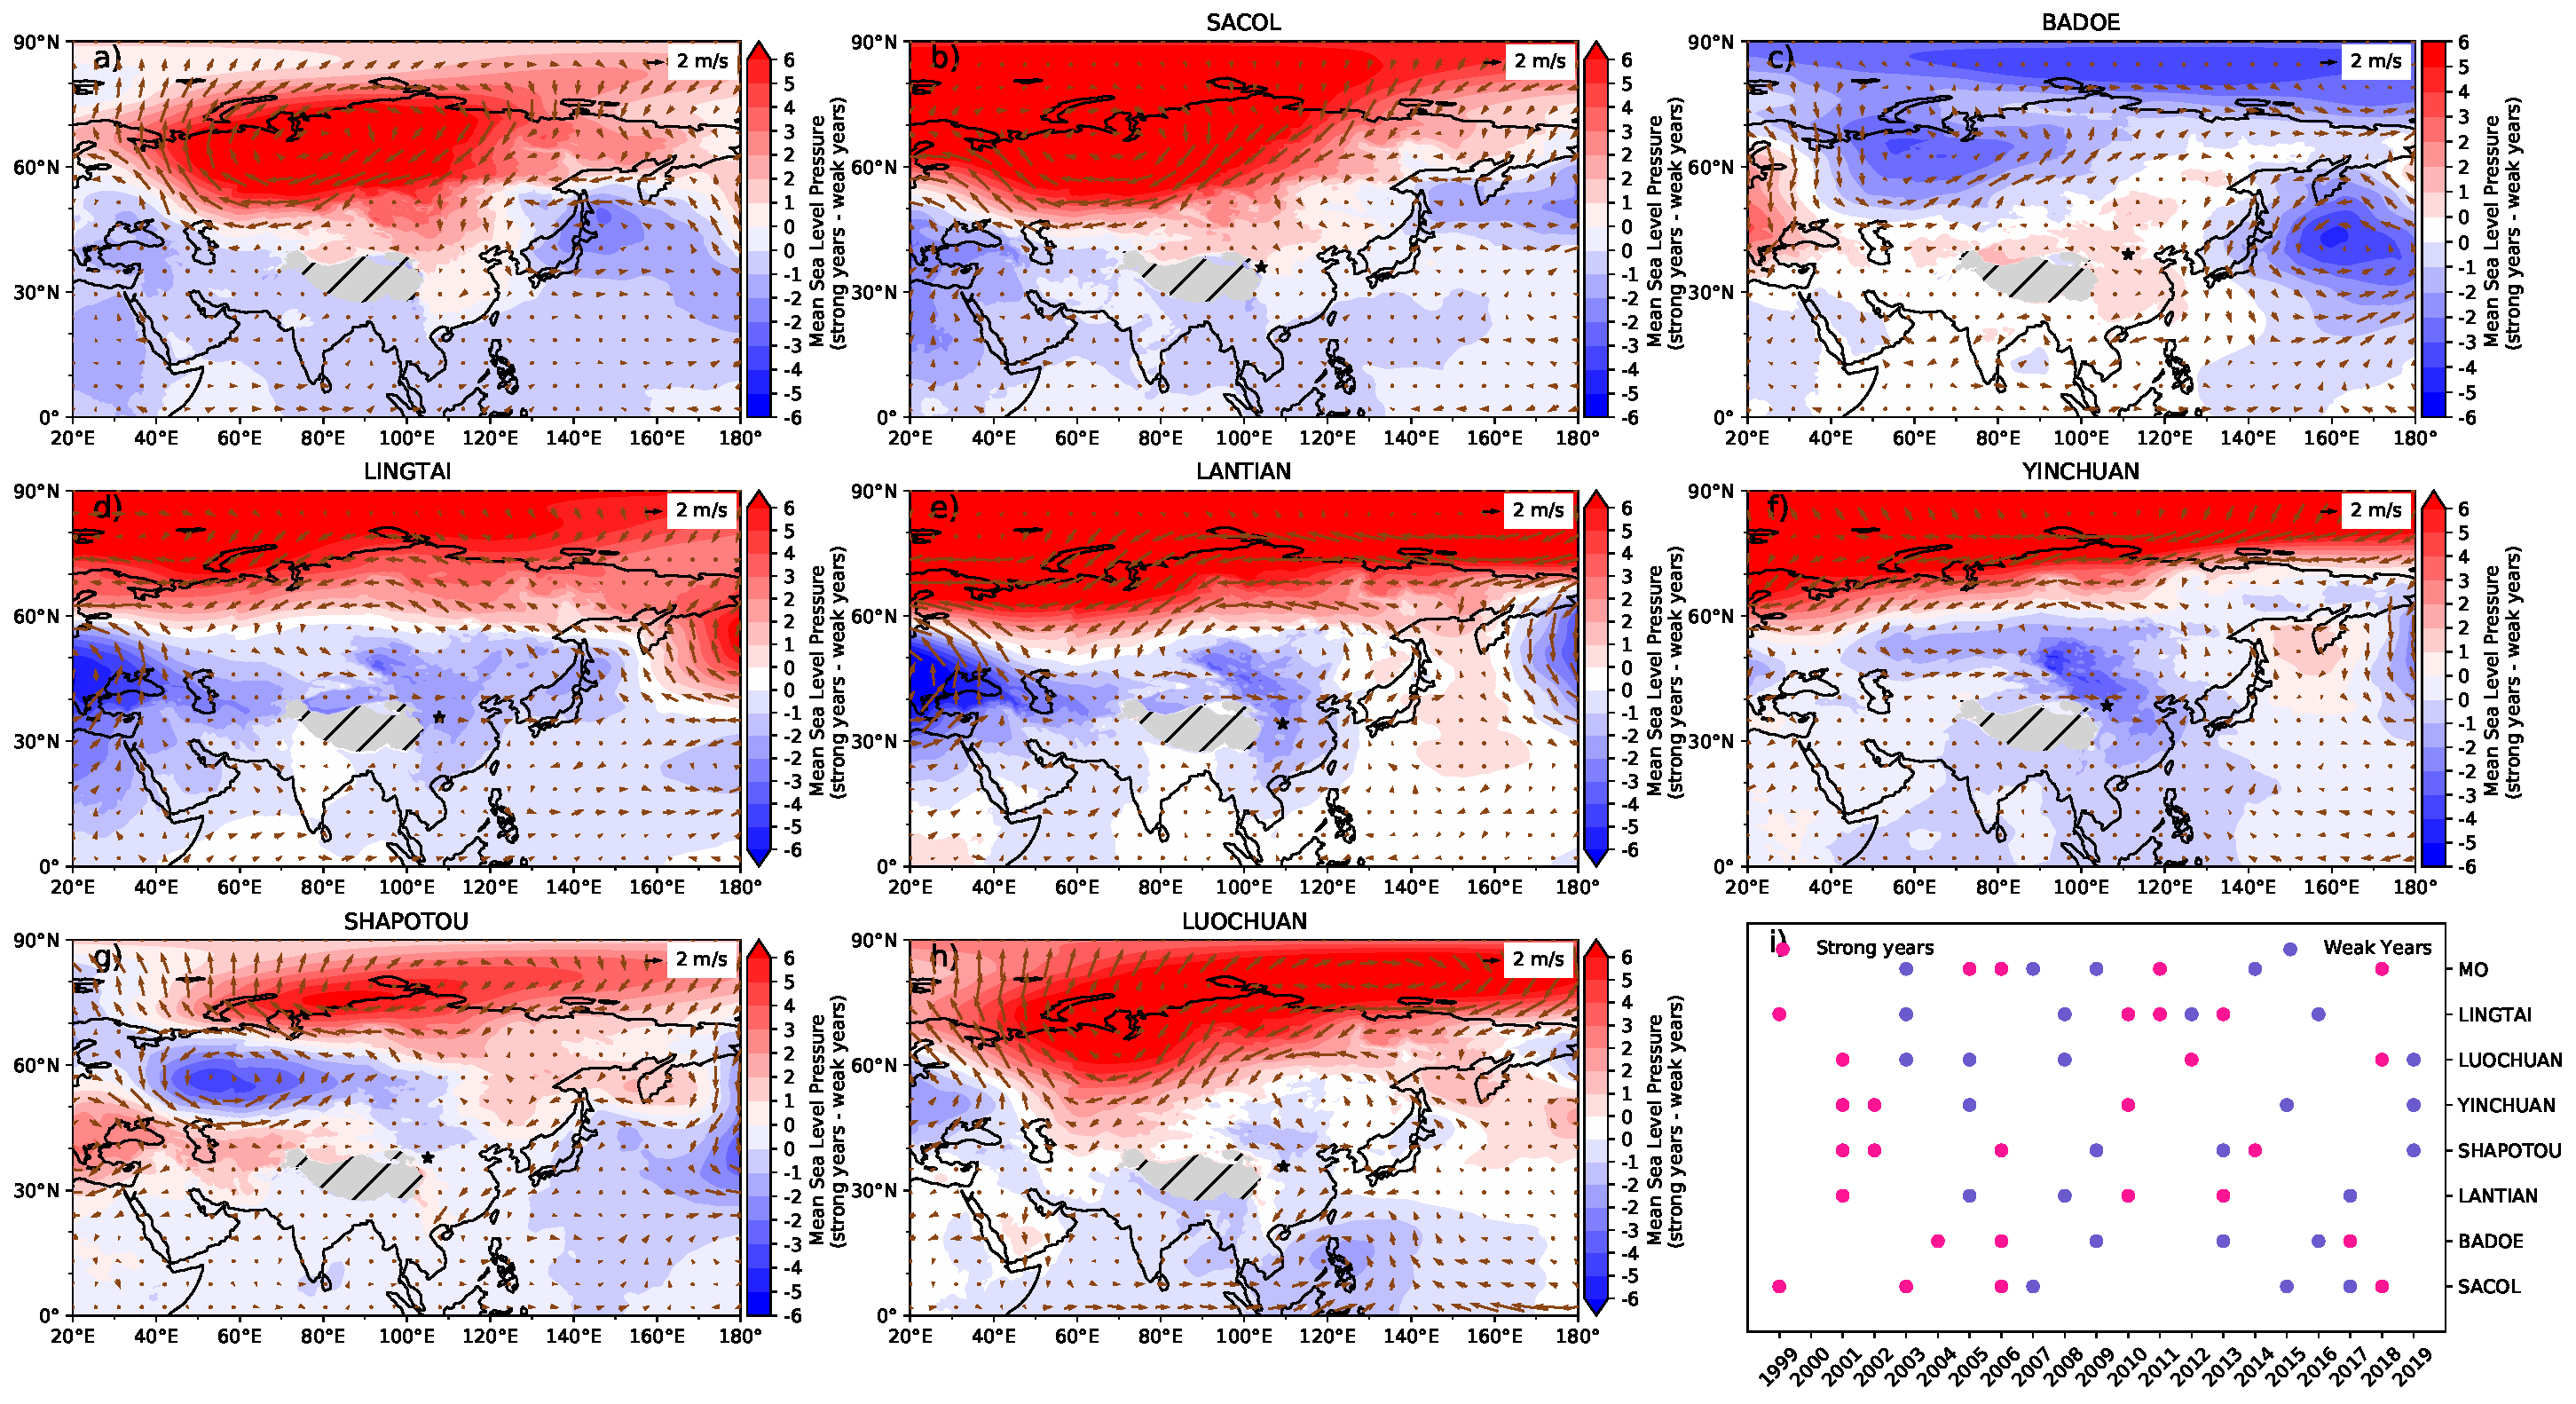
\includegraphics[width=\columnwidth]{texfiles/figs/mslp_850hPa_2micron_DJF.pdf}
    \caption{Composite difference anomalies of mean sea level pressure and 850hPa strong minus weak deposition years of the "fine clay" size bin in winter for all the locations (b-h). (a) is the composite difference anomalies of the strong minus weak winter monsoon years. (i) indicates which years are strong years and which years are weak . Selection of strong and weak years are done according to $\pm$ 1 standard deviation around the mean}
    \label{fig:DJF_850_fine_composite}
\end{sidewaysfigure}